\documentclass{article}

\usepackage{cancel}
\usepackage{amsmath}
\usepackage[includehead,nomarginpar]{geometry}
\usepackage{graphicx}
\usepackage{amsfonts} 
\usepackage{verbatim}
\usepackage{mathrsfs}  
\usepackage{lmodern}
\usepackage{braket}
\usepackage{bookmark}
\usepackage{fancyhdr}
\usepackage{romanbarpagenumber}
\usepackage{minted}
\usepackage{fancyvrb}  % per verbatim in algebra relazionale
%\usepackage{subfig}
\usepackage[italian]{babel}
\usepackage{float}
%\usepackage{wrapfig}
%\usepackage[export]{adjustbox}
\allowdisplaybreaks

\setlength{\headheight}{12.0pt}
\addtolength{\topmargin}{-12.0pt}
\graphicspath{ {./Immagini/} }

\hypersetup{
    colorlinks=true,
    linkcolor=black,
}

\newsavebox{\tempbox} %{\raisebox{\dimexpr.5\ht\tempbox-.5\height\relax}}


\makeatother

\numberwithin{equation}{subsection}
\newcommand{\tageq}{\tag{\stepcounter{equation}\theequation}}
\AtBeginDocument{%
  \renewcommand{\figurename}{Fig.}
}
\fancypagestyle{link}{\fancyhf{}\renewcommand{\headrulewidth}{0pt}\fancyfoot[C]{Sorgente del file LaTeX disponibile al seguente link: \url{https://github.com/00Darxk/Basi-di-Dati/}}}

\begin{document}

\title{%
    \textbf{Basi di Dati}  \\ 
    \large Appunti delle Lezioni di Basi di Dati \\
    \textit{Anno Accademico: 2024/25}}
\author{\textit{Giacomo Sturm}}
\date{\textit{Dipartimento di Ingegneria Civile, Informatica e delle Tecnologie Aeronautiche \\
Università degli Studi ``Roma Tre"}}

\maketitle
\thispagestyle{link}

\clearpage


\pagestyle{fancy}
\fancyhead{}\fancyfoot{}
\fancyhead[C]{\textit{Basi di Dati - Università degli Studi ``Roma Tre"}}
\fancyfoot[C]{\thepage}
\pagenumbering{Roman}

\tableofcontents

\clearpage
\pagenumbering{arabic}

\section{Introduzione}

Per definire cosa sono i dati, si utilizza la definizione del Data Governance Act; per ``Data'' si intende una qualsiasi rappresentazione di informazione. 
Una base di dati in generale, invece, rappresenta un insieme organizzato di dati utilizzati per il supporto dello svolgimento delle attività. La maggior parte delle 
attività moderne si basano su una qualche base di dati. 
Si possono analizzare dal punto di vista metodologico e tecnologico. La definizione dell'Informatica dall'Accademia di Francia si può notare la presenza di queste due 
anime. L'informatica viene definita come la scienza del trattamento razionale, specialmente per mezzo di macchine, dell'informazione considerata come supporto alla 
conoscenza umana e della comunicazione. 



I dati quindi nei sistemi informatici, e non solo, sono mezzi per poter gestire dell'informazione, rappresentati in modo essenziale. Molto spesso vengono rappresentati 
in forma di codice numerico. Sono necessari quindi meccanismi di codifica e decodifica dei dati per poterli rappresentare in forma essenziale e quindi in modo da 
ottenere informazioni. Un dato può essere considerato quindi un elemento di informazione che deve essere ancora elaborato. 

Nello specifico una base di dati rappresenta un insieme organizzato di dati, gestiti da un DBMS. 
Un ``DataBase Management System'' rappresenta un sistema che gestisce collezioni di dati, grandi, persistenti e condivise. 
Si tratta di insiemi grandi, molto di più della memoria fisica dei dispositivi centrali di calcolo, rappresentano il loro limite fisico, e poiché la richiesta di immagazzinare dati 
è sempre maggiore, si vuole aumentare la disponibilità di memorizzare più dati. 
I DBMS sono persistenti, poiché le informazioni salvate al loro interno non svaniscono nel tempo, sono importanti vengono salvati su memorie secondarie non volatili. 
Sono accessibili perché sono condivise e permettono accessi in remoto, essendo generalmente salvati nel cloud. 

I DBMS garantiscono privatezza, affidabilità, efficienza ed efficacia. I DBMS sono privati, poiché devono garantire che i dati salvati al loro interno siano privati, 
e siano accessibili solamente quando vengono richiesti. Devono comprendere meccanismi di autorizzazione per mantenere la privacy. 
Sono affidabili poiché devono poter resistere a malfunzionamenti o attacchi, di tipo hardware o software. I dati sono risorse pregiate e devono poter essere conservati 
a lungo termine. 
Per interfacciarsi con un DBMS una tecnica fondamentale consiste nelle transazioni. Queste sono un insieme di operazioni da considerare indivisibili o atomiche, anche 
concorrenti e di effetto definitivo. Poiché sono operazioni atomiche, possono essere eseguite solo per intero, quando vengono eseguite. Devono essere concorrenti, poiché 
accedendo allo stesso DB da remote bisogna che l'effetto delle due transizioni concorrenti sia coerente sul DB, senza recare danni o perdita di informazioni da nessuna delle 
due. 
I risultati delle transazioni devono essere permanenti ed il loro termine viene identificato da un ``commit'', un impegno che segna una conclusione positiva. Una serie 
di commit quindi mantiene traccia dei risultati in modo definitivo, anche in presenza di guasti o esecuzioni concorrenti. 
L'efficacia e l'efficienza del DBMS dipende da sistema a sistema. 

I progettisti e realizzatori di un DBMS compiono un ruolo diverso dai futuri utilizzatori del DBMS. I primi creano un sistema di gestione, mentre la creazione della base 
di dati è affidati ad altri progettisti. Questa base di dati verrà utilizzata da altri programmatori per realizzare un'applicazione o programma con cui si potranno 
interfacciare gli utenti. Gli utenti finali si distinguono in utenti finali, per cui è stata realizzata quella specifica applicazione ed eseguono operazioni 
predefinite. Mentre utenti casuali eseguono operazioni non previste dal sistema, e possono provocare errori. 

\clearpage

\section{Modello Relazionale}

Per organizzare i dati all'interno di una base di dati si possono utilizzare diversi modelli o astrazioni dei dati. Il modello dei dati rappresenta un insieme di costrutti 
attraverso i quali i dati di interesse vengono organizzati ed utilizzati. Il modello relazionale prevede la costruzione di una tabella, ovvero una relazione, che 
permette di definire insiemi di record o n-uple composte da unità atomiche, chiamate attributi, omogenee. 

Questo rappresenta un modello logico dei dati tradizionale, mentre altri modelli più recenti ad oggetti, XML e ``NoSQL''. 
Il modello relazionale è stato proposto da E. F. Codd nel 1970 per favorire l'indipendenza dei dati. Questo modello fu implementato in DBMS già nel 1981, poiché non è 
facile implementare l'indipendenza dei dati con efficienza ed affidabilità. Si basa sul concetto matematico di relazione che trova una naturale rappresentazione per 
mezzo di tabelle. 

\subsection{Relazione}

Una relazione $\rho$ rappresenta un sottoinsieme del prodotto cartesiano tra due o più domini $D_1$ e $D_2$:
\begin{equation*}
    \rho\subseteq D_1\times D_2
\end{equation*}
Dati $n$ insiemi $D_i$, il loro prodotto cartesiano $D_1\times\cdots\times D_n$ rappresenta l'insieme di tutte le n-uple $(d_1,\cdots,d_n)$ tali che per ogni $i=1,\cdots n$ 
si ha $d_i\in D_i$. Poiché è un insieme non sono presenti ennuple uguali. Una relazione $\rho$ su questi $n$ insiemi, chiamati domini, rappresenta un sottoinsieme 
di questo prodotto cartesiano:
\begin{equation}
    \rho\subseteq D_1\times\cdots\times D_2
\end{equation}

La struttura così definita non è posizionale, poiché a ciascun dominio si associa un nome, attributo o colonna, nell'intestazione della tabella. 
Le tabelle che rappresentano una relazione l'ordinamento tra le righe è irrilevante, così come l'ordinamento tra le colonne. 
Una tabella rappresenta una relazione se tutte le righe sono diverse fra di loro e rappresentano una ennupla distinta, le intestazioni delle colonne sono diverse 
fra di loro, ed i valori di ogni colonna sono omogenei fra di loro. 
Nelle tabelle ci sono solo valori, si indica anche come modello basato sui valori. I riferimenti fra dati in relazioni diverse sono rappresentati tramite i valori 
dei domini nelle ennuple. 

Una base di dati rappresenta un'insieme di relazioni, dove il suo schema è costituito da tutte le intestazioni, mentre i valori contenuti quindi tutte le righe 
contenute nelle tabelle rappresentano un'istanza della base di dati. 

Per gestire le relazioni useremo il linguaggio SQL, inizialmente acronimo per ``Structured English Query Language'', ma poi estesa a ``Structured Query Language'', 
senza appoggiarsi principalmente sul linguaggio inglese. Rappresenta una lingua di alto livello, che tratteremo approfonditamente in sezioni successive. 

Lo schema di una relazione è composto da un nome $R$ ed un insieme $X$ di $n$ attributi $A_i$:
\begin{equation}
    R(A_1,\cdots,A_n)
\end{equation} 
Lo schema di una base di dati $R$ è costituito da uno schema di relazioni $R_i$:
\begin{equation}
    R=\left\{R_1(X_1),\cdots R_k(X_k)\right\}
\end{equation}

Un'ennupla su un insieme di attributi $X$ viene definita come una funzione che associa a ciascun attributo $A$ in $X$ un valore del dominio di $A$. 
Il valore di una singola ennupla $t$ su un attributo $A$ si indica con $t[A]$. Un'istanza di una relazione $\rho$ su uno schema $R(X)$ rappresenta un insieme di 
ennuple su $X$. 
Un'istanza di una base di dati su uno schema $R(X)=\left\{R_1(X_1),\cdots R_k(X_k)\right\}$ si definisce come un insieme di relazioni $\rho=\left\{\rho_i,\cdots,\rho_k\right\}$, 
dove ogni $\rho_i$ rappresenta un'istanza di una relazione sullo schema di una relazione $R_i(X_i)$. 

\subsection{Valore Nullo}

Questo modello impone ai dati una struttura rigida, solo alcuni formati sono infatti ammessi, ed esclusivamente rappresentati come ennuple che appartengono un 
certo schema di relazione. Ma la realtà potrebbe non corrispondere alla struttura attesa, quindi i dati ottenuti dalla realtà potrebbero non rappresentare 
un'ennupla intera. 
Per cui quando un'ennupla contiene informazioni incomplete, il valore dell'ennupla per quell'attributo è vuoto nella relazione. Per ovviare a questo problema nel 
modello relazionale, si utilizza un valore convenzionale per rappresentare questo valore vuoto nell'ennupla, si utilizza un valore diverso dai valori del dominio $A$, 
chiamato $null$. 
L'introduzione di questo altro valore è una soluzione semplice, ma efficace ai fini della base di dati. Tutti i domini $A$ sono in grado di accettare un valore $null$ 
per indicare la mancanza del valore nell'ennupla. Per cui data un'ennupla $t$ il suo valore su di un attributo $A$ può essere:
\begin{equation}
    t[A]=\begin{cases}
        \mathrm{dom}(A)\\
        null
    \end{cases}
\end{equation}


Nonostante la semplicità non è una tecnica perfetta, poiché la perdita di informazioni impedisce di effettuare riferimenti per valori tra le relazioni. 
Su SQL si può utilizzare il comando \verb|NOT NULL| alla creazione di uno schema di relazione. 

\subsection{Vincoli}

Oltre all'assenza di informazioni, è possibile riscontrare errori interni alla base di dati, delle scorrettezze legate all'integrità dei dati. Si possono introdurre 
vincoli di integrità per rappresentare istanze ammissibili. I vincoli sono delle funzioni booleane, dei predicati, che associa ad ogni istanza un valore vero o falso. 

Solo alcuni tipi di vincoli sono integrati nei DBMS, e questi li verificano e ne impediscono la violazione. Per i vincoli supportati invece la verifica spetta all'utente 
o al programmatore. 
Questi vincoli possono essere intra-relazionali o inter-relazionali. I vincoli intra-relazionali coinvolgono solamente i valori di una singola relazione, e possono 
essere sul valore o di dominio, di ennupla, o di chiave. 

\subsubsection{Intra-Relazionali}

I vincoli di dominio impongono condizioni sull'ammissibilità dei valori di un singolo attributo. 
Possono utilizzare operatori booleani come AND, OR e NOT, ed operazioni di confronto matematiche con una costante. 

In SQL data uno schema, si può aggiungere un vincolo con la sintassi \verb|ADD CONSTRAINT|, seguita dalla funzione boolean che definisce il vincolo. Si possono 
aggiungere ad uno schema di relazione tramite il comando \verb|ALTER TABLE|. Se il vincolo che si prova a definire è violato, non si può definirlo. Convenzionalmente 
prima viene definito lo schema con i vincoli poi questi vengono verificati ad ogni modifica, ed in caso rifiutata. 

I vincoli possono essere di ennupla, quando controllano più valori, appartenenti a più attributi, della stessa ennupla. Il vincolo di dominio quindi rappresenta un 
caso particolare del vincolo di ennupla. Rappresenta una combinazione booleana di condizioni semplici sui singoli valori di attributi, due attributi o più valori di essi. 


Se un insieme $K$, dominio della relazione, è una chiave, allora per il vincolo di chiave si impone che non possano esistere due ennuple uguali su $K$. Una chiave 
essendo univoca permette di identificare le ennuple, ed è minimale rispetto a questa proprietà. Ovvero è l'insieme più piccolo possibile per poter identificare univocamente 
tutte le ennuple della relazione. Se una chiave è formata da più di un insieme allora si chiama superchiave. Su SQL si indica che un attributo è una chiave attraverso 
il comando \verb|UNIQUE|. Alcune chiavi possono essere definite su più attributi, ma devono essere univoche. Una chiave è una superchiave minimale. 

Ogni relazione è un insieme, quindi non può contenere due ennuple uguali, e ha come superchiave almeno l'insieme degli attributi su cui è stata definita. Ogni relazione 
ha almeno una chiave. 
L'esistenza delle chiavi garantisce la possibilità di accedere ad ogni ennupla della base di dati e permettono di correlare relazioni diverse. 
Se nella chiave sono presenti valori nulli, questo non permette di identificare le ennuple e di realizzare facilmente riferimenti ad altre relazioni. Per cui la loro 
presenza nelle chiavi deve essere limitata o almeno controllata. 

Una chiave si dice primaria se su di essa non sono ammessi valori nulli, indicata nell'intestazione sottolineando l'attributo corrispondente. 


In SQL dopo aver definito lo schema della relazione, si inserisce la parola chiave \verb|KEY| o \verb|PRIMARY| \verb|KEY|, in seguito all'attributo considerato come 
chiave oppure si inseriscono tra parentesi questi attributi. 

\subsubsection{Inter-Relazionali}

Un vincolo di integrità referenziale, utilizza delle chiavi esterne ``foreign key'' $X$ per collegare due relazioni $R_1$ e $R_2$. Questo vincolo impone ai valori su 
$X$ in $R_1$ di comparire come valori della chiave primaria in $R_2$.  


In SQL si definiscono dopo le colonne degli attribuiti tramite la parola chiave \verb|FOREIGN KEY| specificando tra parentesi gli attributi da considerare. Si 
inserisce in seguito \verb|REFERENCES| seguito dal nome della relazione $R_1$ e tra parentesi gli attributi di questa relazione da utilizzare. 

Quando questi vincoli sono su attributi multipli il loro ordine è rilevante, poiché le chiavi devono riferire agli attributi corretti, altrimenti non sarebbe presente un riscontro tra i domini. La struttura è in 
notazione posizionale. 

Spesso è richiesto che un singolo attributo sia legato ad una relazione, ma all'interno di una tabella, e relazione, è possibile utilizzare solamente valori semplici, non relazioni. 
Per risolvere questa richiesta si utilizzano altre relazioni esterne, connesse utilizzando vincoli referenziali, per realizzare strutture simili a strutture nidificate, in più relazioni. I dati di interesse 
infatti hanno una struttura generalmente nidificata, e per poter essere rappresentati in relazioni hanno bisogno di essere trasformati attraverso vari livelli di astrazione, che rappresentano un diverso livello 
di dettaglio dello stesso fenomeno reale. 
Questo meccanismo verrà trattato dettagliatamente nella sezione dedicata alla progettazione di basi di dati. In molti casi non vengono rappresentati ad una prima analisi tutti gli aspetti significativi di un 
dato reale, e quindi si tende a modificare le relazioni ottenute all'aumentare delle informazioni ottenute dagli stessi dati. 

Ogni modello presenta un suo livello di astrazione, utili per un ristretto contesto, e perde di utilità se viene utilizzato in contesti diversi. Questo vale per ogni modello, le cui informazioni di interesse potrebbero 
o non potrebbero essere utili in base al tipo di analisi ed operazioni da effettuare. 


\clearpage

\section{Algebra Relazionale}

Esistono due diversi tipi di linguaggi per basi di dati, rispetto alla loro funzione. Si può operare sullo schema della base di dati tramite DDL ``Data Definition Language'', oppure sui dati 
memorizzati, tramite DML ``Data Manipulation Language''. Con la DML è possibile effettuare interrogazioni o ``query'' sul database ed operazioni di aggiornamento.

I linguaggi DML, interrogativi, per basi di dati relazionali possono essere dichiarativi, ovvero esprimono le proprietà del risultato che si cerca, oppure possono essere procedurali ed indicano il modo in cui 
si ottiene il risultato di interesse. 

Alcuni di questi linguaggi sono:
\begin{itemize}
    \item Algebra Relazionale: procedurale;
    \item Calcolo Relazionale: dichiarativo, e teorico;
    \item SQL: parzialmente dichiarativo, di uso reale;
    \item QBE: dichiarativo, di uso reale. 
\end{itemize} 

L'algebra relazionale fornisce un linguaggio tramite il cui è possibile effettuare interrogazioni su basi di dati, è quindi un linguaggio di tipo DML. Contiene un insieme di operatori su relazioni, che producono 
una relazione. Quindi questi operatori possono essere composti l'uno sull'altro. 
In questo corso verrà utilizzato il servizio online RelaX per utilizzare l'algebra relazionale. Questo sistema fornisce una struttura ad albero dell'interrogazione, dove le foglie sono gli operandi ed i 
nodi interni gli operatori. Per effettuare un'interrogazione dato il suo albero, si parte dalle foglie, e si sale al loro genitore e si effettua questa operazione, salendo di un solo nodo alla volta, arrivando 
fino alla radice dove sarà presente la relazione risultato dell'interrogazione. 

L'algebra relazionale definisce i seguenti operatori:
\begin{itemize}
    \item Unione, Intersezione e Differenza;
    \item Ridenominazione;
    \item Selezione;
    \item Proiezione;
    \item Aggregazione;
    \item Join. 
\end{itemize}

\subsection{Operatori Insiemistici}

Sono disponibili operatori essenziali per insiemi, poiché le relazioni corrispondono a degli insiemi. Poiché i risultati devono essere relazioni, si possono applicare solamente su relazioni aventi gli stessi 
attributi. Questa condizione però è mitigabile. 
Queste operazioni sono l'unione tra due relazioni, l'intersezione e la differenza. La relazione risultante presenta gli stessi attributi, nello stesso ordine degli operandi, con un numero di ennuple che dipende 
dal tipo di operazione. Ogni ennupla presente nel risultato deve quindi essere presente in almeno uno degli operandi. 

Su RelaX queste operazioni vengono identificate dai caratteri $\cap$: intersezione, $\cup$: unione e $\setminus$: differenza. 

L'unione tra relazioni aventi attributi diversi non è scorretta logicamente, ma utilizzando l'operatore insiemistico è impossibile. Bisogna gestire in modo corretto i nomi degli 
attributi che si vuole, ed esiste un operatore specifico per effettuarlo. Su RelaX produce un risultato diverso da quello aspettato. 

\subsection{Ridenominazione}

Questo operatore permette di rinominare i nomi degli attributi in una relazione, passati come argomento. Può essere utilizzato per generare un risultato intermedio con attributi omonimi, tra due relazioni diverse, 
per effettuare un'unione. In questo modo la relazione rimane uguale, ma cambiano solamente i nomi, in questo modo l'unione produce risultati comprensibili. 

Questo operatore si indica con $\rho$, REN o RHO. Prende tra parentesi il nome della relazione di cui si vuole modificare il nome, e come pedice indica il vecchio nome e come cambiarlo:
% \begin{equation}
%     \mbox{REN}_{\mathrm{ListaNuoviNomi}\leftarrow\mathrm{ListaVecchiNomi}}(\mathrm{Relazione})
% \end{equation}
\begin{Verbatim}[commandchars=\\\{\}, codes={\catcode`$=3\catcode`_=8}]
    REN\textsubscript{\texttt{ListaNuoviNomi}$\leftarrow$\texttt{ListaVecchiNomi}}($R$)
\end{Verbatim}

Si possono rinominare più di un attributo alla volta, specificando come pedici la lista degli attributi. Entrambe le liste nei pedici devono essere ordinate correttamente per poter agire sugli attributi specificati. 

\subsection{Selezione}

Questo operatore selezione da una relazione, le ennuple che soddisfano una certa condizione, sui loro attributi. Questo operatore si indica con $\sigma$ o \verb|SEL|, e si rappresenta la condizione tramite una funzione 
booleana sul pedice, applicata su tutte le ennuple della relazione passata come argomento. Se questa condizione è verificata per una certa ennupla, questa viene selezionata ed appartiene al risultato, altrimenti non 
viene considerata. 
Effettivamente realizza tagli orizzontali della tabella associata alla relazione. Si utilizza la seguente sintassi:
% \begin{equation}
%     \mathrm{SEL}_{\mathrm{{Condizione}}}(\mathrm{Relazione})
% \end{equation}
\begin{Verbatim}[commandchars=\\\{\}, codes={\catcode`$=3\catcode`_=8}]
    SEL\textsubscript{\texttt{Condizione}}($R$)
    $\sigma$\textsubscript{\texttt{Condizione}}($R$)
\end{Verbatim}
Nella condizione booleana si possono effettuare confronti matematici tra attributi e costanti, e si possono utilizzare operatori booleani come \verb|AND|, \verb|OR| e \verb|NOT|. 
Quando su un attributo sono possibili valori nulli, le condizioni producono risultati un risultato non desiderabile, poiché le condizioni atomiche vengono valutate separatamente. In generale nei linguaggi per basi 
di dati sono necessarie operazioni aggiuntive per gestire valori nulli, come \verb|IS NULL| e \verb|IS NOT NULL|. Senza queste operazioni si dovrebbe utilizzare la relazione senza considerare gli attributi dove possono essere 
presenti attributi nulli. 
Si potrebbe ulteriormente utilizzare una logica a tre stati, con uno stato sconosciuto per condizioni su attributi nulli. In RelaX si usa la sintassi:
% \begin{equation}
%     \mathrm{NomeAttributo}=\mathrm{null}
% \end{equation}
\begin{Verbatim}[commandchars=\\\{\}, codes={\catcode`$=3\catcode`_=8}]
    NomeAttributo = NULL
\end{Verbatim}
\subsection{Proiezione}

La proiezione è un'operazione che seziona verticalmente una relazione, agisce su tutte le ennuple, e solo sugli attributi specificati. Si indica con $\pi$ o \verb|PROJ|, e prende come argomento tra parentesi la relazione 
su cui agisce, e come pedice una lista di attributi:
% \begin{equation}
%     \mathrm{PROJ}_{\mathrm{ListaAttributi}}(Relazione)
% \end{equation}
\begin{Verbatim}[commandchars=\\\{\}, codes={\catcode`$=3\catcode`_=8}]
    PROJ\textsubscript{\texttt{ListaAttributi}}($R$)
    $\pi$\textsubscript{\texttt{ListaAttributi}}($R$)
\end{Verbatim}
Il risultato è una relazione contenente tutte le ennuple ottenute dalla relazione di partenza ristrette agli attributi specificati nella lista. Rappresenta quindi un'operazione ortogonale rispetto 
alla selezione. Poiché rimuove gli attributi non presenti nella lista, è possibile siano presenti ennuple identiche nel risultato. 

La cardinalità di una proiezione indica il numero di ennuple del risultato dell'operazione. Può contenere un numero minore di ennuple rispetto all'operando. Se la lista di attributi coincide, o contiene una 
superchiave $X$ della relazione $R$ allora l'operazione:
\begin{Verbatim}[commandchars=\\\{\}, codes={\catcode`$=3\catcode`_=8}]
    $\pi_X$($R$)
\end{Verbatim}
Contiene esattamente lo stesso numero di ennuple della relazione $R$, e non sono presenti ennuple duplicate. 


La selezione e la proiezione sono operatori che permettono di estrarre informazioni da una relazione, restringendo le ennuple, e gli attributi. Effettuando una decomposizione orizzontale e verticale. 
Non è possibile invece calcolare calcolare informazioni derivate, oppure correlare fra di loro informazioni presenti in relazioni diverse. 

\subsection{Join}

L'operatore join è l'operatore più interessante fornito dall'algebra relazionale. Permette di correlare informazioni presenti su più relazioni, tra di loro. Effettua quest'operazione congiungendo 
ennuple di relazioni diverse su attributi dello stesso nome. 

Il join è quindi un operatore binario, generalizzabile, e produce un risultato sull'unione degli attributi degli operandi. Le ennuple del risultato sono costruite a partire da ciascuna ennupla degli operandi. 

Si definisce l'operatore join naturale $\Join$ tra due relazioni $R_1$ e $R_2$ su insiemi di attributi rispettivamente $X_1$ e $X_2$:
\begin{equation}
    R_1(X_1)\Join R_2(X_2)=\left\{t\,\mbox{su}\,X_1X_2\,\mbox{t.c.}\,\exists \,t_1\in R_1\land t_2\in R_2\implies t[X_1]=t_1\land t[X_2]=t_2\right\}
\end{equation} 

Un join si dice completo, se ogni ennupla contribuisce al risultato, mentre un join vuoto produce una relazione vuota, poiché non è possibile combinare tra di loro le ennuple delle due relazioni di partenza. 
Ha una cardinalità massima data dalla cardinalità delle due relazioni $R_1$ e $R_2$, nel caso di un join completo, mentre ha una cardinalità minima pari a zero, nel caso di un join vuoto:
\begin{equation}
    0\leq |R_1\Join R_2|\leq |R_1|\cdot|R_2|
\end{equation} 

Se il join coinvolge una chiave di $R_2$ allora, produrrà al massimo $|R_1|$ ennuple differenti, poiché la relazione considera al massimo tutte le ennuple di $R_2$, associandole con le ennuple di $R_1$:
\begin{equation*}
    0\leq |R_1\Join R_2|\leq |R_1|
\end{equation*}

Invece se il join coinvolge una chiave di integrità referenziale tra le due relazioni $R_1$ e $R_2$, allora conterrà esattamente un numero $|R_1|$ di ennuple, senza contenere duplicati:
\begin{equation*}
    |R_1\Join R_2|=|R_1|
\end{equation*}

In generale la cardinalità di un join è intermedia a questi valori di cardinalità, dove una parte delle ennuple non contribuisce al risultato finale, vengono tagliate fuori. 
Se si vuole considerare anche queste ennuple, allora si può utilizzare il join esterno, che che estende il join, utilizzando valori nulli. Si indica dove aggiungere queste ennuple tagliate fuori, ed il resto degli 
attributi, non presenti in una delle due relazioni vengono attribuiti pari a null. 

Esiste in tre versioni: sinistro, destro e completo. Il tipo di join esterno si indica al pedice del comando \verb|JOIN|. Il join esterno sinistro, considera solo le ennuple della relazione $R_1$ e le aggiunge al 
risultato, quello esterno analogamente solo $R_2$, mentre quello completo da entrambe. 

%% TODO join e proiezioni

Un join naturale su una relazione senza attributi in comune si definisce prodotto cartesiano, contiene sempre un numero di ennuple pari al prodotto delle cardinalità delle due relazioni. Si suppone che le ennuple 
sono tutte combinabili tra di loro. Il risultato contiene ogni possibile combinazione tra tutte le ennuple degli operandi. 
Viene utilizzato in genere sempre se seguito da una condizione booleana, tramite una selezione:
% \begin{equation*}
%     \mbox{SEL}_{\mbox{Condizione}}(R_1\Join R_2)
% \end{equation*}
\begin{Verbatim}[commandchars=\\\{\}, codes={\catcode`$=3\catcode`_=8}]
    SEL\textsubscript{\texttt{Condizione}}($R_1\Join R_2$)
    $\sigma$\textsubscript{\texttt{Condizione}}($R_1\Join R_2$)
\end{Verbatim}
Quest'operazione viene chiamata ``theta-join'', e può essere espressa specificando la condizione al pedice del join. Se la condizione nel theta-join comprende sempre l'uguaglianza, allora questo si chiama 
``equi-join''. Si utilizzano sopratutto equi-join e non theta-join. L'equi-join è definito quindi come il prodotto cartesiano tra due relazioni, seguito da una selezione all'uguaglianza, tra due liste di attributi 
di entrambe le relazioni. Viene utilizzato per correlare due attributi di nome diverso, ma di stesso valore. 
Nelle interrogazioni pratiche si userà solamente l'equi-join, mentre il join naturale viene descritto esclusivamente ad uso didattico. 

Due espressioni si dicono equivalenti se producono risultati uguali in ogni istanza della base di dati, è rilevante poiché i DBMS utilizzano forme equivalenti per ridurre la complessità e rendere le interrogazioni 
più efficienti. 
Una di queste forme equivalenti è la ``push selection'', una selezione all'uguaglianza di un attributo con una costante su una join tra due relazioni. Questa forma è equivalente ad eseguire la selezione prima della 
join, sulla relazione contenente l'attributo di interesse. 

Tuttavia l'obiettivo di questo corso non è l'efficienza delle interrogazioni, ma la loro correttezza, dato che sono i DBMS a decidere quale sia la scelta più efficiente, e ad eseguirla. 

\subsection{Viste}

Date questi operatori è possibile realizzare altre relazioni, non contenute nella base di dati operando su di esse, e correlando le informazioni contenute al loro interno. Le relazioni appartenenti all'istanza 
della base di dati si chiamano relazioni di base. Le relazioni definite attraverso interrogazioni vengono chiamate relazioni derivate, queste possono essere definite su altre relazioni derivate. Ma questo processo 
di realizzare interrogazioni nidificate o annidate può rendere meno comprensibile l'interrogazione. 

L'uso delle viste non influisce sull'efficienza dell'interrogazione. Nelle interrogazioni ci si riferisce alle viste come fosse una relazione appartenente alla base di dati. Rappresentano uno strumento di 
programmazione per diminuire il codice ripetuto e semplificare la scrittura di interrogazioni. 

Inoltre questa distinzione permette agli utenti di poter interagire solamente con ciò che gli interessa, o che sono autorizzati a vedere. Permette inoltre l'utilizzo di programmi esistenti su schemi 
ristrutturati. 

\subsection{RelaX}

RelaX è uno strumento online per effettuare interrogazioni in algebra relazionale. 

La sintassi è molto simile a quella descritta nel libro di testo, anche se presenta piccole differenze. L'editor permette di cliccare su un'operazione ed inserirla, in una barra 
sopra la zona di interrogazione. L'editor è ``case sensitive'', quindi bisogna prestare attenzione alle maiuscole. 
A volte le espressioni perdono di leggibilità, poiché non è possibile inserire le condizione al pedice, vanno infatti inserite tutte su una singola linea. A volte lo strumento si confonde sugli spazi, ed è 
consigliabile utilizzarne di più oppure utilizzare parentesi ampiamente. 

Fornisce anche una rappresentazione grafica ad albero delle espressioni, di facile comprensione. 

Accedendo al servizio si possono effettuare interrogazioni su basi di dati, caricate dall'utente, oppure preesistenti sul servizio. Per caricare una base di dati, si può specificare nel link URL per accedere al 
servizio, oppure caricandola nel group editor. 
La sintassi per descrivere una relazione è la seguente: prima si specifica il nome della relazione, assegnando con un uguale la sua istanza tra parentesi graffe. All'interno delle parentesi graffe la prima 
riga indica i nomi degli attributi della relazione, divisi da spazi. Accanto al nome si può specificare il tipo di dato accettato da quell'attributo, dopo dei due punti. Se non viene specificato sarà possibile 
utilizzare qualunque tipo. Nelle righe seguenti si popola la base di dati specificando per ogni riga un'ennupla diversa, con i valori separati da spazi. 

Nelle interrogazioni è consigliabile inserire nei confronti per primo l'attributo del primo operando e per secondo l'attributo del secondo operando. 

Quando vengono effettuate operazioni di join tra due relazioni con attributi di nome uguale, si comporta essenzialmente come SQL. Viene ignorato il join naturale, e per riconoscere gli attributi viene utilizzato 
in notazione puntata il nome della relazione di appartenenza. Per rinominare relazioni si utilizzano viste, poiché rinominare attributi singoli è molto verboso ed è strettamente necessario solamente quando 
bisogna effettuare delle unioni, o per dare nomi significativi nel risultato. In RelaX è necessaria una ridenominazione esplicita prima dell'assegnazione alla vista, tramite l'operatore $\rho$. 

\clearpage

\section{SQL}

Esistono diversi tipi di linguaggi per accedere alle basi di dati. Già si è analizzata l'algebra relazionale, un linguaggio procedurale, per costruire gradualmente il risultato tramite le relazioni della 
base di dati. 

Il linguaggio SQL ``Structured Query Language'', si basa in parte sull'algebra relazionale, mentre su altri aspetti è un linguaggio dichiarativo, spesso permette di specificare nelle interrogazioni la struttura e le 
proprietà del risultato, a partire delle relazioni della base di dati. Ora SQL non rappresenta più un acronimo, ma solo un nome arbitrario.  
Il linguaggio tende ad essere sintetico ed abbastanza intuitivo per certi aspetti. 

Ne esistono varie versioni, standard fino ad un certo punto, ed è un linguaggio molto grande, e ne verranno analizzate solo funzioni generali. 
Si può definire la componente di costruzione dei dati, e la componente di manipolazioni dei dati nello stesso SQL. 

Ogni versione di SQL presenta dei piccoli dettagli diversi, ma che impediscono la completa esecuzione di una interrogazione arbitraria per un altro sistema. Il sistema utilizzato durante il corso è un servizio 
online chiamato \href{https://sqliteonline.com/}{SQLiteonline}, con una base di dati sul cloud. 
Su questo servizio è possibile utilizzare diverse DBMS SQL, oltre alla versione SQLite, si utilizzerà anche PostgreSQL, poiché fornisce un linguaggio più completo. 
Poiché è un servizio web, le basi di dati analizzate vengono salvate nella cache e quindi dovranno essere inizializzate ogni volte che vi si accede. 

Nel servizio web, alla sinistra sono presenti, oltre a vari DBMS, la basi di dati corrente, alla destra è presente la storia delle precedenti interrogazioni. Al centro è presente l'interfaccia dove si possono 
scrivere le interrogazioni. Il risultato apparirò a schermo sotto questo editor, ma non verrà inserito all'interno della base di dati. 


SQL è indifferente tra maiuscolo e minuscolo per i suoi comandi, ma è preferibile essere coerente con le scelte di sintassi effettuate. Inoltre è indifferente 
dall'indentazione, ma si preferisce inserire parentesi oppure si va a capo per aumentare la leggibilità dell'interrogazione. Il linguaggio lo 
interpreta cercando il nome della parola chiave, e gli argomenti dell'interrogazione.  


\subsection{DDL}

Per creare uno schema di qualsiasi tipo si utilizza la parola chiave \verb|CREATE|, seguito dal tipo di oggetto da creare. Nella maggior parte dei casi si realizzeranno solamente relazioni, o tabelle, di tipo 
\verb|TABLE|. In seguito viene inserito il nome della relazione, e tra parentesi tonde si inserisce ad ogni riga il nome dell'attributo della relazione e le sue proprietà:
\begin{minted}{sql}
CREATE TABLE NomeRelazione (
    NomeAttributo1 TipoAttributo1 VincoliAttributo1, 
    -- lista di attributi
    NomeAttributoN TipoAttributoN VincoliAttributoN,
    -- definizioni opzionali di superchiavi della relazione
);
    
-- creazione degli altri schemi della base di dati
\end{minted}

Tra i tipi possibili si hanno numeri specificati dalla parola chiave \verb|number|, date da \verb|date|, stringe di caratteri di una certa lunghezza \verb|character(n)|, etc. Tra i vincoli di un attributo si 
può specificare se non deve essere nullo tramite il costrutto \verb|NOT NULL|, di default quindi un attributo può assumere come valore \verb|NULL|. Se esiste una chiave primaria, si può specificare direttamente nel 
campo proprietà di un attributo, invece che alla fine delle dichiarazioni di attributi. Si può specificare un vincolo di integrità referenziale tramite la parola chiave \verb|REFERENCES|, seguito dal nome dell'attributo, 
se univoco, oppure dal nome della relazione che lo contiene, seguito tra parentesi tonde il suo nome, se non univoco. 

In molti sistemi si possono utilizzare strumenti diversi da SQL per realizzare schemi di relazioni, il sistema PgAdmin offre un'interfaccia grafica. Ma è preferibile utilizzare il linguaggio SQL in modo da 
essere riutilizzabile, e di implementazione più veloce. 
In alcuni DBMS, se non viene specificato che la chiave primaria sia diversa da \verb|NULL|, questi sistemi utilizzano un valore progressivo di default, quando non viene inserito esplicitamente dall'utente.  


Per i nomi delle relazioni o degli attributi si utilizzano solo lettere minuscole, senza accenti. Invece dello spazio, se necessario, si può utilizzare il carattere \verb|_| nei nomi. 

Con la parola chiave \verb|SELECT| si effettuano delle interrogazioni sui dati, mentre si possono modificare i dati con \verb|INSERT|, \verb|DELETE| e \verb|UPDATE|. 
Con \verb|INSERT| è possibile inserire una nuova riga in una relazione si utilizza la sintassi:
\begin{minted}{sql}
INSERT INTO NomeRelazione (ListaAttributi) -- omessa se coinvolge tutti gli attributi, o nello stesso ordine
    VALUES (ListaValori) -- specificati tra singoli apici e divisi da una virgola
\end{minted}
Invece di specificare i valori tramite \verb|VALUES|, è possibile utilizzare \verb|SELECT|, ma verrà discusso più avanti. Se un attributo non è presente nella lista, il suo valore in quell'ennupla inserita sarà 
\verb|NULL|. 


In SQL si possono scrivere operazioni di aggiornamento del database, tramite il comando \verb|INSERT INTO|, allo stesso modo si possono eliminare dei valori con 
\verb|REMOVE FROM|. Per modificare una tabella già creata, si può utilizzare il comando \verb|ALTER TABLE|. Si possono rimuovere relazioni, o altri oggetti, specificando il loro nome nella clausola \verb|DROP TABLE|. 


In SQLiteonline l'inserimento di una ennupla in una tabella non controlla se gli attributi con cui hanno un vincolo di integrità referenziale che si vogliono aggiungere sono presenti nella relazione 
a cui si riferiscono, altrimenti potrebbe causare dei danni all'intera base di dati. Questa reference dovrebbe essere controllata ad ogni inserimento. 

Su SQLite si può attivare il controllo della chiave esterna con il comando:
\begin{minted}{sql}
    PRAGMA foreign_keys=on
\end{minted}

\subsection{DML}

In SQL si possono effettuare le stesse operazioni disponibili nell'algebra relazionale, utilizzando una sintassi diversa:

\subsubsection{Proiezione}

Per visualizzare alcuni attributi da una relazione, si può utilizzare una proiezione, introdotta dalla parola chiave \verb|SELECT|, seguita dalla lista di attributi di interesse. Anche se si vuole visualizzare l'intera 
relazione bisogna usare una proiezione, specificando come parametro \verb|*|, per indicare di visualizzare tutti gli attributi. Per specificare a quale relazione si vuole effettuare la proiezione, si utilizza 
la parola chiave \verb|FROM|, seguita dal nome della relazione:
\begin{minted}{sql}
    SELECT ListaAttributi -- oppure '*'
    FROM NomeRelazione
\end{minted}

La lista di attributi si indica anche come ``target list'', su cui devono operare condizioni, clausole, o funzioni più complesse, trattate in seguito. 

\subsubsection{Operatori Insiemistici e Ridenominazione}

Nell'algebra queste operazioni devono essere effettuate sugli stessi schemi, ma il loro comportamento è leggermente diverso tra RelaX e SQL. L'unione si effettua tramite la parola chiave \verb|UNION|, tramite 
due interrogazioni, dove si richiedono gli stessi attributi:
\begin{minted}{sql}
    SELECT ListaAttributi
    FROM Relazione1
    UNION
    SELECT ListaAttributi
    FROM Relazione2
\end{minted}

Il risultato è una nuova tabella con tutte le righe di entrambe le tabelle. Se nelle due relazioni gli attributi sono differenti è possibile realizzare un'unione forzata, mentre nell'algebra solamente se i due 
insiemi sono uguali. In base al DBMS utilizzato è possibile effettuare unioni tra relazioni con numero di attributi differente, gestiti in maniera automatica. Questo però richiede ennuple compatibili tra di loro. 
Si utilizza l'approccio posizionale, nella lista degli attributi della proiezione. In questo modo si può specificare quali attributi unire tra di loro nell'unione. Inserisce prima tutte le ennuple della prima relazione, 
ed in seguito concatena, se sono compatibili, tutte le ennuple nell'ordine di attributi specificato della seconda relazione. 
Quindi in molti sistemi quest'operazione non è commutativa, il risultato prodotto sarà differente in base a quale relazione viene inserita per prima. Poiché il nome degli attributi nella relazione finale dipende 
solo dalla prima relazione. 
La maggior parte dei DBMS non vengono controllai se i nomi degli attributi combaciano, quindi bisogna prestare attenzione sopratutto all'ordine in cui sono inseriti nell'interrogazione ed al loro nome. 

Per rinominare degli attributi si utilizza la parola chiave \verb|AS| nella lista degli attributi della proiezione. Questo può essere omesso, inserendo solamente il nome dell'attributo ed il nome del suo alias:
\begin{minted}[mathescape, escapeinside=||]{sql}
    SELECT NomeAttributo1 AS NomeAlias1, |$\cdots$|, NomeAttributoN NomeAliasN
    FROM Relazione
\end{minted}

Come nell'algebra relazionale, rinominando gli attributi è possibile realizzare l'unione, anche se in algebra relazionale è possibile solamente dopo una ridenominazione. L'ordine rimane comunque importante, 
nonostante la ridenominazione. Si può quindi realizzare una proiezione con ridenominazione, nella stessa interrogazione. 

Quando in un'interrogazione non si è sicure del risultato, l'ambiguità deve essere risolta a monte. 

Nell'unione, poiché si tratta di insiemi, le ennuple identiche verranno eliminate nella relazione risultante. Si può specificare con \verb|UNION ALL| di mantenere tutti i duplicati tra le due relazioni su cui 
viene effettuata l'unione. 


La differenza viene realizzata tramite il comando \verb|EXCEPT|:
\begin{minted}{sql}
    SELECT ListaAttributi
    FROM Relazione1
    EXCEPT
    SELECT ListaAttributi
    FROM Relazione2
\end{minted}

Produce una relazione contenente tutte le ennuple della prima relazione, eccetto le ennuple contenute anche nella seconda relazione. Come per l'intersezione il comportamento di SQL è analogo all'algebra relazionale. 
Si specifica l'intersezione tra due relazioni con la parola chiave \verb|INTERSECT|:
\begin{minted}{sql}
    SELECT ListaAttributi
    FROM Relazione1
    INTERSECT
    SELECT ListaAttributi
    FROM Relazione2
\end{minted}

\subsubsection{Selezione}

Per specificare una condizione su un'interrogazione si inserisce una riga al termine dell'interrogazione introdotta dalla parola chiave \verb|WHERE|, seguita dalla funzione booleana che si deve verificare:

\begin{minted}{SQL}
    SELECT ListaAttributi
    FROM Relazione
    WHERE Condizione
\end{minted}

Questa interrogazione una selezione ed una proiezione, per la lista di attributi passata come argomento alla \verb|SELECT|. 

\subsubsection{Join}

Il join essenzialmente realizza un prodotto cartesiano delle relazioni specificate nella clausola \verb|FROM|: 
\begin{minted}{sql}
    SELECT *
    FROM Relazione1 JOIN Relazione2
\end{minted}

Può essere specificata una condizione dalla parola chiave \verb|WHERE|, se si cercano solo certi attributi, si può effettuare una proiezione specificando la lista di attributi dopo 
la parola chiave \verb|SELECT|. In SQL bisogna specificare con la parola chiave \verb|DISTINCT| se si vuole avere solo ennuple diverse tra di loro: 
\begin{minted}{sql}
    SELECT DISTINCT ListaAttributi
    FROM Relazione1 JOIN Relazione2
    WHERE Condizione
\end{minted}


In algebra relazionale è possibile scrivere interrogazioni equivalenti in modi diversi, in cui ci sono variazioni di efficienza, 
l'algebra è procedurale. In SQL invece il sistema si preoccupa dell'efficienza delle operazioni, è almeno in parte dichiarativo dove le interrogazioni 
possono essere scritte in modi diversi, ma alcune differenze presenti in algebra non emergono. 


Il sistema esegue selezione join ed un ulteriore proiezione, nella versione base di SQL. QUalche anno dopo venne introdotto il join esplicito, 
introducendo la possibilità di specificare i join nella clausola \verb|FROM| specificando l'argomento al posto di una lista di attributi, una lista 
di join effettuati su attributi, specificando la condizione di join dopo la clausola \verb|ON|. 

Date due relazioni contenente un attributo in comune, per realizzare una relazione di join su questo attributo in comune si specifica nella 
clausola \verb|SELECT| l'attributo in notazione puntata, altrimenti solleverebbe un errore poiché rappresenta un nome ambiguo. Anche nella 
condizione di join nella clausola \verb|FROM| bisogna specificare a chi appartiene l'attributo indicato, utilizzando la notazione puntata: 

\begin{minted}{SQL}
    SELECT Attributo1, Attributo2, Lista1.AttributoComune 
    --oppure anche Lista2.AttributoComune
    FROM Lista1 JOIN Lista2 ON Lista1.AttributoComune = Lista2.AttributoComune
\end{minted}

In SQL esiste il modo per effettuare join naturali specificando il nome dell'attributo non in notazione puntata, utilizzando la clausola \verb|USING|, 
ma è preferibile non usarlo per favorire la comprensione:

\begin{minted}{SQL}
    SELECT AttributoComune, Attributo1, Attributo2
    FROM Lista1 JOIN Lista2 USING AttributoComune
\end{minted}

Alternativamente è possibile utilizzare più volte la stessa relazione in un'interrogazione, applicando una ridenominazione dei suoi attributi. In questo modo è possibile eliminare le ambiguità generate effettuando diversi 
join sulle stesse relazioni. 

Questo è utile per visualizzare campi dallo stesso nome, ridenominando gli attributi del risultato, oppure per facilitare la scrittura 
evitando nomi di relazioni molto lunghi. 

Esiste in SQL il join esterno, dove alcuni degli operandi partecipano solamente in parte, tramite la clausola \verb|LEFT|, \verb|RIGHT| o \verb|FULL| 
seguito da \verb|JOIN|. Inoltre è possibile inserire \verb|OUTER| per realizzare join equivalenti, ma queste funzioni non sono presenti nel servizio web SQLite, dove 
è possibile utilizzare solamente \verb|LEFT JOIN|. 

\subsubsection{Condizioni ``Like''}

L'ordinamento del risultato è un altro fattore determinante, in base a cui si distinguono due ennuple 
o soluzioni tra di loro. Si può effettuare operazioni sulla target list e si può utilizzare la condizione \verb|LIKE| per identificare espressioni regolari, dove 
\verb|_| identifica un qualsiasi carattere e \verb|%| per qualsiasi sequenza di carattere, inseriti tra doppi apici \verb|" ... "|. 

\subsubsection{Aggregazione ed Operatori Aggregati}

Il contenuto delle basi di dati viene spesso aggregato, ma questo non è possibile in algebra relazionale. SQL prevede la possibilità di calcolare piccole elaborazioni 
a partire da insiemi di ennuple, di conteggio, minimo, massimo, media o totale. 

Queste operazioni vengono svolte da operatori aggregati quali \verb|COUNT| per contare tutti le righe in una relazione. Le funzioni aggregative 
lavorano anche con valori nulli. Bisogna specificare l'attributo di cui contare tutte le righe nella relazione tra parentesi tonde:
\begin{minted}{SQL}
    COUNT(Attributo)
\end{minted}
Altri operatori aggregati sono \verb|SUM|, \verb|AVG|, \verb|MAX| e \verb|MIN|. Si nota un'ulteriore utilità del valore nullo, poiché il sistema li 
riconosce come un valore non reale e non lo utilizza nel calcolo, al contrario di un sistema dove i valori nulli vengono codificati con 0 o -1. 

Si utilizza un'altra clausola \verb|GROUP BY| per dividere le ennuple di una relazione sulla base dell'attributo specificato e su questi raggruppamenti viene eseguita la funzione 
aggregata specificata. Quando si raggruppa su un attributo, e per lo stesso valore sono presenti più di un valore, è presente un'ambiguita su quale valore da visualizzare. Su SQLite viene mostrato uno scelto 
casualmente tra questi attributi. Questa rappresenta una delle scorrettezze di SQLite, ed il motivo per cui utilizzare spesso raggruppamenti viene sconsigliato. Questo può sollevare un 
problema quando è richiesto individuare un massimo su un attributo in una relazione, se si utilizza questo costrutto, e sono presenti più di un attributo con lo stesso valore massimo, allora 
sarà mostrato solo uno, riportando un risultato errato rispetto ai dati di partenza. Su altri DBMS questo problema può essere risolto restituendo un insieme delle ennuple che soddisfano 
l'interrogazione specificata.  

Per ordinare una relazione si può utilizzare la clausola \verb|ORDER BY|, seguita dall'attributo su cui si deve effettuare l'ordinamento. 

Esiste un altra clausola \verb|HAVING| per definire una condizione su raggruppamenti, mentre la \verb|WHERE| si usa sulle singole ennuple. 

\subsubsection{Interrogazioni Nidificate e Viste}

La funzioni di aggregazione effettuano l'operazione sulla target list, raggruppando i campi, quindi in alcuni casi non permettono di scegliere di quale ennupla mostrare 
l'attributo. Si applicano al gruppo di ennuple che soddisfano la condizione imposta dal \verb|GROUP BY|. 
Per risolvere questo problema e non perdere informazioni sulle relazioni utilizzati, si può utilizzare una vista, oppure interrogazioni nidificate. Le viste sono 
interrogazioni, calcolata per mezzo di un'espressione, utilizzabile come fosse una relazione. Prima di creare una vista è consigliabile 
effettuare l'interrogazione per osservare il suo risultato. 
In SQL non esistono valori, ma relazioni di singolo attributi su una singola ennupla. 

All'interno di un'interrogazione è possibile scrivere altre interrogazioni, in molti modi diversi nella versioni recenti di SQL. Si può inserire nei comandi \verb|WHERE|, 
\verb|FROM|, \verb|SELECT|, etc. Esiste anche con i tipi, per esempio con valori booleani con \verb|EXISTS|. 

Se nel \verb|WHERE|, invece di restituire una ennupla con un singolo valore dalla sotto-interrogazione, vengono restituite diverse ennupla, in SQLite questo non genera 
un errore, ma rappresenta un comportamento errato della piattaforma. Su PostgreSQL infatti questo solleva un errore, poiché non può utilizzare le ennuple fornite nel 
confronto. In questo modo è come se l'interrogazione interna nella \verb|WHERE|, utilizzando attributi dell'interrogazione esterna, venga eseguita ogni volta per ogni 
ennupla della interrogazione esterna. 

Le interrogazioni nidificate erano nella versione base di SQL, fin dalla sua nascita, poiché non si credeva di poter utilizzare la join. Quindi ogni interrogazioni 
veniva realizzata con valori distinti, ma si capì molto presto la necessità di introdurre la join per effettuare interrogazioni più semplicemente. 

\clearpage

\section{Progettazione di Basi di Dati}

La progettazione di un'applicazione consiste nel definire lo schema logico della base di dati. Questo schema può essere definito direttamente se la base di dati è 
semplice, ma quando comincia ad essere complessa è facile perdersi nei dettagli senza averne un quadro di insieme. Il modello relazionale è anche abbastanza rigido, 
quindi quest'operazione richiede passaggi anche molto complessi. 

A seconda del livello del dettaglio si possono rappresentare più o meno aspetti dello stesso fenomeno, introducendo più attributi in una stessa relazione, oppure 
utilizzando più relazioni. 
Inoltre è necessario fin da subito conoscere come relazionare le varie tabelle tra di loro. 

La progettazione di una basi di dati rappresenta un'attività ragionevolmente organizzata in cui si segue un metodo per costruire in modo solido, sapendo quello che 
si costruisce. \`{E} una delle attività del processo di sviluppo dei sistemi informativi. Un sistema informativo è un insieme di attività, realizzazioni informatiche 
ed organizzative per supportare certe attività. La realizzazione di questi sistemi comporta molte attività complesse tra di loro interconnesse, non nettamente 
separate. Le fasi di realizzazione trattate in questo corso sono la raccolta ed analisi dei requisiti e la progettazione e le problematiche relative a queste attività. 

La progettazione di un sistema informativo riguarda gli aspetti di progettazione dei dati e delle applicazioni, su cui è possibile interagire con questi dati. I dati 
hanno spesso un ruolo centrale in queste applicazioni, sono stabili. 


La progettazione viene divisa in quattro fasi, una prima fase di progettazione concettuale per determinare le caratteristiche dei dati che si vuole andare a memorizzare 
e gestire nella base di dati. Questa prima fase viene chiamata analisi. Nelle fasi successive di progettazione concettuale si determina come vengono effettivamente 
modellati e gestiti i dati all'interno della base di dati.  

Prima di determinare i dati bisogna determinare i concetti su cui opera la base di dati, è necessario identificare una realtà di interesse di cui si vuole modellare 
i dati. 

Prima di definire lo schema logico si determina lo schema concettuale per determinare la realtà di interesse da modellare. Nel corso della progettazione si avranno 
diversi prodotti:
\begin{itemize}
    \item Schema concettuale;
    \item Schema logico;
    \item Schema fisico. 
\end{itemize}

Lo schema fisico non verrà trattato in questo corso. Lo schema logico è già stato trattato precedentemente e rappresenta l'insieme delle relazioni che definiscono 
la base di dati. 

Il modello dei dati è un insieme di costrutti utilizzati per memorizzare i dati. Lo schema relazionale consiste in una serie di relazioni, rappresentate come tabelle. 
Esistono due tipi principali di modelli dei dati, uno logico, comprende il modello relazionale, reticolare, a oggetti, etc; ed uno concettuale. 
Ci sono molti modelli concettuali, e tante varianti, il più noto è il modello ``Entity-Relationship''

\subsection{Il Modello ER: Schema Concettuale}

Il modello ER rappresenta il modello concettuale più diffuso, ne esistono diverse versioni con qualche differenza tra l'una e l'altra. Prevede una serie di costrutti:
\begin{itemize}
    \item Entità: classi di oggetti della realtà di interesse con proprietà comuni e con esistenza ``autonoma'', in modo che i singoli oggetti siano riconoscibili;
    \item Relationship: un legame logico fra due o più entità, rilevante nell'applicazione di interesse;
    \item Attributo;
    \item Identificatore;
    \item Generalizzazione. 
\end{itemize}

Ad un'entità nel modello ER corrisponde probabilmente una relazione nel modello relazionale. 
Per il modello ER si utilizza anche una rappresentazione grafica, che sarà utilizzata molto nell'ambito di questo corso. Le entità vengono rappresentate come dei 
rettangoli, mentre le relationship come dei rombi. 

\begin{figure}[H]%
    \centering%
    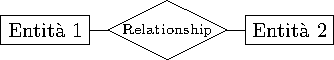
\includegraphics[scale=1.25]{entita_relationship.pdf}%
\end{figure}

Come per le relazioni esiste uno schema ed un'istanza per le entità. Invece di istanza si utilizza il termine occorrenza di un entità per rappresentare un singolo 
elemento di quella classe, definita dall'entità. Nel modello concettuale si rappresentano le entità, non le singole occorrenze, rappresenta un livello di astrazione. 
Ogni entità ha un nome che la identifica univocamente nello schema, ha bisogno di nomi espressivi. 


Una relationship è un legame logico tra due o più entità, è possible chiamarlo relazione, anche se non coincide con il concetto di relazione nel modello relazionale. 
Convenzionalmente si utilizza il singolare e sostantivi, non verbi, per identificare le relationship con un nome univoco. 

Un'occorrenza di una relationship è una coppia tra un'occorrenza di un'entità ed un'occorrenza di un'altra entità. Ogni relationship ha un insieme di occorrenze, quindi 
non ci possono essere coppie di entità ripetute sulla stessa relationship. Invece è possibile che le stesse due entità siano connesse da più relationship.   
Bisogna quindi modellare entità e relationship rispetto alla realtà di interesse per non avere coppie ripetute. Per rappresentare coppie ripetute in un modello ER, si 
``promuove'' la relazione a livello di entità e si collega alle entità precedenti con due nuove relationship. 

Il concetto di relationship non è strettamente binario, ma potrebbero esistere relationship n-arie, anche se la maggior parte delle relationship non coinvolge più di tre 
entità, e già relationship ternarie sono rare. 
Possono coesistere diverse relationship che coinvolgono le stesse entità. Inoltre possono esistere relationship ricorsive, che coinvolgono più volte la stessa entità, 
ed in queste viene associato un ruolo ad ognuno di questi due utilizzi dell'entità. Quando si incontrano delle relationship non corrette, generalmente vengono promosse ad entità per rappresentare 
quella caratteristica della realtà di interesse. 

Esiste anche il costrutto di attributo, rappresenta una proprietà elementare di un'entità o di una relationship, di interesse ai fini dell'applicazione. Associa ad ogni 
occorrenza di un'entità un valore appartenente ad un insieme di dominio. Ma questo non rappresenta lo scopo principale del modello concettuale, quindi è un elemento 
di secondo livello nella progettazione concettuale. 

\begin{figure}[H]%
    \centering%
    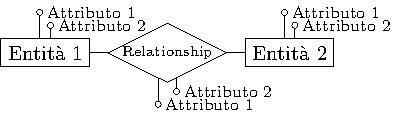
\includegraphics[scale=1.25]{entita_relationship_attributo.pdf}%
\end{figure}

Si possono utilizzare attributi composti, definiti come un'insieme di attributi di una stessa entità per rappresentare meglio l'informazione. 

\begin{figure}[H]%
    \centering%
    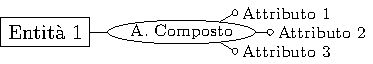
\includegraphics[scale=1.25]{entita_attributo_composto.pdf}%
\end{figure}
Altri costrutti per precisare meglio gli schemi concettuali sono la cardinalità, di relationship o entità, una coppia di valori utilizzati per determinare il numero 
massimo e minimo delle relationship cui ciascuna occorrenza di un'entità può partecipare. 

Per semplicità si utilizzano solamente tre simboli: 0, 1 e ``N''. Si utilizza 0 ed 1 per la cardinalità minima, con zero si ha una partecipazione opzionale, mentre 
con 1 si ha una partecipazione obbligatoria. Mentre si usa 1 o N per la massima, con N si indica che non sono presenti limiti superiori al numero di occorrenze. 

Rispetto a queste cardinalità massime le relationship possono essere definite:
\begin{itemize}
    \item Uno a Uno: $(x,1)$-$(x,1)$;
    \item Uno a Molti: $(x,1)$-$(x,N)$;
    \item Molti a Molti: $(x, N)$-$(x, N)$. 
\end{itemize}

Se un attributo individua un concetto interessato di cui si vuole rappresentare altre 
caratteristiche bisogna promuoverlo ad entità, così come altri costrutti del modello ER. Quando un attributo viene promosso ad entità si dice che viene ``reificato'', ovvero ci si interessa del concetto individuato dall'attributo. 

Le relationship di cardinalità obbligatoria per entrambe le entità sono molto rare. 
Per le relationship uno a molti esiste un'altra notazione sconsigliata per rappresentare la cardinalità:

\begin{figure}[H]%
    \centering%
    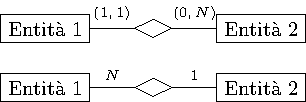
\includegraphics[scale=1.25]{notazione_uno_molti.pdf}%
\end{figure}

Si può inserire la cardinalità anche sugli attributi. Queste rappresentano delle opzionalità, poiché l'informazione potrebbe essere incompleta, oppure per specificare degli attributi multivalore, 
raramente utilizzati. In questo corso non verranno quasi mai utilizzati attributi multivalore. 
\begin{figure}[H]%
    \centering%
    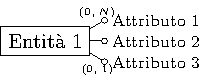
\includegraphics[scale=1.25]{attributo_cardinalita.pdf}%
\end{figure}

Sulle entità si può inserire un identificatore per determinare in maniera univoca le occorrenze dell'entità, può essere costituito da attributo delle entità, 
identificatore interno, oppure da altre entità tramite relationship, identificatore esterno. Talvolta è necessario utilizzare più di un attributo e si indica come una barra che 
attraversa tutti gli attributi che sono coinvolti: 
\begin{figure}[H]%
    \centering%
    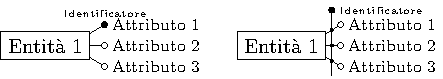
\includegraphics[scale=1.25]{identificatore_interno.pdf}%
\end{figure}

A volte non è sufficiente utilizzare un identificatore interno, poiché il concetto dipende da caratteristiche di altri concetti. Un identificatore esterno si rappresenta 
come un arco che attraversa sia l'attributo interno che la relationship che lega l'entità che permette l'identificazione. 
Questo è possibile solamente se la relationship a cui è collegato ha una cardinalità minima pari ad uno, inoltre anche la cardinalità massima deve essere pari ad uno 
per avere una relazione univoca per identificare l'entità: 

\begin{figure}[H]%
    \centering%
    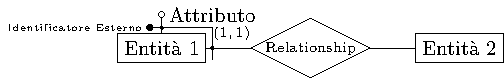
\includegraphics[scale=1.25]{identificatore_esterno.pdf}%
\end{figure}

\`{E} consigliabile utilizzare almeno un identificatore per 
ogni entità. Possono essere presenti più identificatori su una 
stessa entità, sia interni che esterni, disgiunti tra di loro. Se sono presenti altri identificatori la cardinalità 
dell'identificatore esterno può anche essere opzionale e non 
obbligatoria. 



Ci sono casi dove è utile indicare sottoinsiemi di una stessa entità, si utilizza una freccia come notazione grafica, che punta dal sottoinsieme all'entità base. 
Questo costrutto si chiama generalizzazione, mette in relazione una o più entità, con un entità che le comprende, come casi particolari. Si dice che le entità $E_1,\cdots,E_n$ sono 
sottotipi o specializzazioni dell'entità $E$. Questo approccio riprende dalla programmazione orientata agli oggetti. 
Ogni occorrenza dei sottotipi è anche un'occorrenza dell'entità base, tutte le proprietà dell'entità genitore sono valide anche per le entità figlie. Per proprietà 
si intendono tutti gli attributi e tutte le relazioni. 

Talvolta può essere utile distinguere diversi tipi di generalizzazioni. Si dice generalizzazione totale se ogni occorrenza del genitore è occorrenza di almeno 
una delle entità figlie, altrimenti è parziale:
\begin{figure}[H]%
    \centering%
    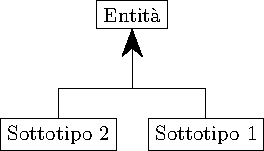
\includegraphics[scale=1.25]{generalizzazione_totale.pdf}%
\end{figure}
Si dice esclusiva se ogni occorrenza del genitore è occorrenza di al più una delle entità figlie, 
altrimenti si dice sovrapposta:
\begin{figure}[H]%
    \centering%
    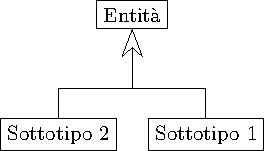
\includegraphics[scale=1.25]{generalizzazione_esclusiva.pdf}%
\end{figure}
Si considerano senza perdita di generalità solo generalizzazioni esclusive e si distingue tra generalizzazioni parziali e totali. 
Se sono esclusive in termini insiemistici le entità figlie hanno intersezione nulla. 

Una generalizzazione può esistere a gerarchie a più livelli, e multiple generalizzazioni allo stesso livello. Una stessa entità può appartenere a più gerarchie come genitore e/o figlia. Una generalizzazione con una singola entità 
figlia si chiama sottoinsieme. 

Per progettare bisogna fornire una documentazione per riuscire ad operare, gestire e manutenere la base di dati. 
Per definire uno schema ER bisogna fornire un dizionario dei dati, e dei vincoli non esprimibili nello schema, queste sono proprietà non rappresentabili con uno 
schema ER, ma che appartengono alla realtà di interesse analizzata. 
Il dizionario dei dati elenca ed anche descrive le proprietà di tutte le entità e relazioni, si riporta il nome, una descrizione testuale, gli attributi e 
l'identificare. 
Analogamente alle entità si ha una descrizione delle relazioni, i suoi componenti ed eventuali attributi.

\subsection{Progettazione Concettuale}

%% TODO inizio lezione 15/11/24

Questa fase di acquisizione ed analisi dei requisiti è difficile, anche difficile da standardizzare e da insegnare. Non è un'operazione che segue 
passi strettamente tecnici, richiede molta esperienza. 

Si effettua una raccolta di dati preliminare. Gli utenti possono fornire informazioni e possono fornire una visione ad alto livello, ma non dettagliata, oppure 
dettagliata, ma di basso livello. Queste interviste portano ad un acquisizione che richiede un ulteriore acquisizione per raffinare i dati ottenuti. 

Insieme al cliente si chiede di determinare definizioni e classificazioni, e si prova a determinare aspetti essenziali rispetto a quelli marginali. 

Tutto ciò che viene raccolto da queste interrogazioni viene essere inserito in una documentazione descrittiva, scegliendo il giusto livello di astrazione. 
Standardizzando la struttura delle frasi, suddividendole in frasi semplice. Si separano le frasi sui dati dalle operazioni sui dati. Una volta ottenuti i dati ci si 
preoccupa che i dati siano definiti in maniera corretta. 

Vanno organizzati termini e concetti tramite un glossario. Questi rappresentano entità e relazioni nel modello. Si individuano sinonimi ed omonimi per semplificare il 
linguaggio. Si rende esplicito il riferimento tra i vari termini. E si riorganizza tra concetti. 

Per ristruttura in gruppi omogenei la documentazione si individuano frasi di carattere generale, e si cercano di individuare tutte le frasi relative ad uno specifico 
concetto, e si dividono rispetto a questi concetti. 

Sulla base di questo si prova a determinare quale costrutti assegnare in base alle caratteristiche dei concetti. Se hanno proprietà significative e 
descrive oggetti con esistenza autonoma si rappresentano con entità. 


Alcuni oggetti possono ripetersi in concetti diversi 

%% TODO add lezione 15/11/24

\subsection{Progettazione logica}

%% TODO add inizio lezione 22/11/24


Molti dei costrutti dello schema E-R sono direttamente associabili ad elementi del modello relazionale. 
Gli identificatori rappresentano chiavi nel modello relazionale, dove le entità e le relationship rappresentano le singole relazioni. Invece di inserire una relazione per 
ogni relationship si potrebbe inserire una attributo in una delle relazioni che lega con un vincolo di integrità referenziale ad un attributo dell'altra relazione connessa 
dalla relationship. Altrimenti se la cardinalità della relationship non lo permette si deve necessariamente realizzare come una relazione, con attributi che legano entrambe 
le entità della relationship. In questo caso la chiave è costituita da questi attributi, poiché ogni istanza di una relationship deve essere unica. Si realizza in questo 
modo quando si hanno relationship molti a molti, invece se si hanno relationship uno a molti, non è necessario utilizzare una tabella. 
Inoltre attributi con una cardinalità massima superiore ad uno si realizzano come relazioni, con un vincolo di integrità referenziale all'entità di appartenenza. 

%% TODO ex corrispondenze 

Nel caso in cui ci siano delle generalizzazioni, non sono presenti costrutti che le traducono direttamente. %% TODO img generalizzazione
Potrebbero essere presenti ridondanze nei dati, concettualmente si vogliono poche ripetizioni, ma alcune potrebbero essere utili. Queste ridondanze potrebbero essere 
caratteristiche direttamente calcolabili dalle relazioni già presenti. Se l'attributo ridondante è poco richiesto, si potrebbe non inserire, mentre se bisogna 
accedere spesso a questa caratteristica, è conveniente utilizzare una attributo. Ma in questo modo è necessario aggiornare l'attributo a ogni aggiornamento dei dati 
su cui si basa su altre relazioni. Se gli aggiornamenti costano meno delle interrogazioni sono convenienti le ridondanze, ma questo suppone di conoscere il carico sulla 
base di dati. Bisogna conoscere il tipo di operazioni che verranno applicate sulla base di dati, e quindi il modello logico che si vuole utilizzare, in in questo caso 
il modello relazionale. 

Si considerano degli indicatori, lo spazio che occupa in memoria la base di dati, ed il tempo delle occorrenze. %% TODO add indicatori

Ci possono essere ridondanze anche nelle relationship. %% TODO add
per calcolare il costo complessivo si moltiplica la frequenza di una singola operazione per il costo di quell'operazione, per ognuna delle singole operazioni. Quindi 
bisogna fornire la frequenza delle operazioni che si applicano alla base di dati, per la sua progettazione. Considerando questo operazioni ed il suo 
carico in memoria ed in frequenza si realizzano relazioni diverse, mantenendo o eliminando ridondanze. 

Si può decidere di aggregare ciò che viene acceduto insieme e separare ciò che viene acceduto separatamente. In un modello E-R ristrutturato vengono eliminate le 
generalizzazioni sostituendole in entità e relationship. Si può effettuare in tre modi diversi. %% TODO  

%% TODO entità e relationship molti a molti

Come convenzione, sui nomi degli attributi della relazione create da una relationship si utilizzano i nomi delle entità di partenza. Ogni azienda ha le sue convenzioni 
per definire nomi diversi per gli attributi. 

La traduzione non riesce a tener conto delle cardinalità minime, si dovrebbero aggiungere ulteriori vincoli, tramite \verb|CHECK|, non sono molto usati, ma è possibile 
realizzarli in modo molto preciso e rigoroso. Possono esistere relationship ricorsive, dove la relationship viene tradotta in una relazione, con due nomi diversi per 
entrambe le ricorrenze della stessa relazione. 
Se la cardinalità minima è zero, l'attributo deve ammettere valori nulli. 
Se l'identificatore esterno è anche la relationship si inserisce come attributo nella relazione. 

\end{document}